\documentclass[conference]{IEEEtran}
\IEEEoverridecommandlockouts
\usepackage{cite}
\usepackage{amsmath,amssymb,amsfonts}
\usepackage{algorithmic}
\usepackage{graphicx}
\usepackage{textcomp}
\usepackage{xcolor}
\usepackage{booktabs}
\usepackage{url}
\usepackage{microtype}

% Load dynamically generated numbers from raw data predictions
% Auto-generated by experiments/make_numbers.py - DO NOT EDIT MANUALLY
\newcommand{\Datasettotalresponses}{39895}
\newcommand{\Nragtruthtrainresponses}{12690}
\newcommand{\Nragtruthtrainclaims}{99696}
\newcommand{\Prevragtruthtrain}{44.9}
\newcommand{\Nragtruthdevresponses}{2252}
\newcommand{\Nragtruthdevclaims}{17571}
\newcommand{\Prevragtruthdev}{44.6}
\newcommand{\Nragtruthtestresponses}{2675}
\newcommand{\Nragtruthtestclaims}{19861}
\newcommand{\Prevragtruthtest}{35.2}
\newcommand{\Nhaluevalqatrainresponses}{12000}
\newcommand{\Nhaluevalqatrainclaims}{12377}
\newcommand{\Prevhaluevalqatrain}{50.0}
\newcommand{\Nhaluevalqadevresponses}{3000}
\newcommand{\Nhaluevalqadevclaims}{3092}
\newcommand{\Prevhaluevalqadev}{50.0}
\newcommand{\Nhaluevalqatestresponses}{5000}
\newcommand{\Nhaluevalqatestclaims}{5160}
\newcommand{\Prevhaluevalqatest}{50.0}
\newcommand{\Ntruthfulqatrainresponses}{948}
\newcommand{\Ntruthfulqatrainclaims}{957}
\newcommand{\Prevtruthfulqatrain}{50.0}
\newcommand{\Ntruthfulqadevresponses}{236}
\newcommand{\Ntruthfulqadevclaims}{237}
\newcommand{\Prevtruthfulqadev}{50.0}
\newcommand{\Ntruthfulqatestresponses}{396}
\newcommand{\Ntruthfulqatestclaims}{403}
\newcommand{\Prevtruthfulqatest}{50.0}
\newcommand{\Nwikibiogpt3trainresponses}{143}
\newcommand{\Nwikibiogpt3trainclaims}{1127}
\newcommand{\Prevwikibiogpt3train}{95.1}
\newcommand{\Nwikibiogpt3devresponses}{36}
\newcommand{\Nwikibiogpt3devclaims}{302}
\newcommand{\Prevwikibiogpt3dev}{94.4}
\newcommand{\Nwikibiogpt3testresponses}{59}
\newcommand{\Nwikibiogpt3testclaims}{479}
\newcommand{\Prevwikibiogpt3test}{94.9}
\newcommand{\Nfavamultisamplestrainresponses}{267}
\newcommand{\Nfavamultisamplestrainclaims}{3272}
\newcommand{\Prevfavamultisamplestrain}{68.5}
\newcommand{\Nfavamultisamplesdevresponses}{65}
\newcommand{\Nfavamultisamplesdevclaims}{774}
\newcommand{\Prevfavamultisamplesdev}{67.7}
\newcommand{\Nfavamultisamplestestresponses}{128}
\newcommand{\Nfavamultisamplestestclaims}{1614}
\newcommand{\Prevfavamultisamplestest}{62.5}
\newcommand{\Npooledtotaltrainresponses}{26048}
\newcommand{\Npooledtotaltrainclaims}{117429}
\newcommand{\Prevpooledtotaltrain}{47.9}
\newcommand{\Npooledtotaldevresponses}{5589}
\newcommand{\Npooledtotaldevclaims}{21976}
\newcommand{\Prevpooledtotaldev}{48.3}
\newcommand{\Npooledtotaltestresponses}{8258}
\newcommand{\Npooledtotaltestclaims}{27517}
\newcommand{\Prevpooledtotaltest}{45.7}
\newcommand{\Aucharmoniq}{0.800}
\newcommand{\Auclowharmoniq}{0.711}
\newcommand{\Auchighharmoniq}{0.879}
\newcommand{\Balaccharmoniq}{0.713}
\newcommand{\Fprharmoniq}{26.5}
\newcommand{\Fnrharmoniq}{31.0}
\newcommand{\Eceharmoniq}{0.088}
\newcommand{\Brierharmoniq}{0.193}
\newcommand{\Aucminicheck}{0.782}
\newcommand{\Auclowminicheck}{0.703}
\newcommand{\Auchighminicheck}{0.870}
\newcommand{\Balaccminicheck}{0.643}
\newcommand{\Fprminicheck}{0.0}
\newcommand{\Fnrminicheck}{71.4}
\newcommand{\Eceminicheck}{0.227}
\newcommand{\Brierminicheck}{0.246}
\newcommand{\AucvectaraHhem}{0.755}
\newcommand{\AuclowvectaraHhem}{0.674}
\newcommand{\AuchighvectaraHhem}{0.839}
\newcommand{\BalaccvectaraHhem}{0.548}
\newcommand{\FprvectaraHhem}{0.0}
\newcommand{\FnrvectaraHhem}{90.5}
\newcommand{\EcevectaraHhem}{0.278}
\newcommand{\BriervectaraHhem}{0.288}
\newcommand{\Aucalignscore}{0.782}
\newcommand{\Auclowalignscore}{0.703}
\newcommand{\Auchighalignscore}{0.870}
\newcommand{\Balaccalignscore}{0.643}
\newcommand{\Fpralignscore}{0.0}
\newcommand{\Fnralignscore}{71.4}
\newcommand{\Ecealignscore}{0.227}
\newcommand{\Brieralignscore}{0.246}
\newcommand{\Aucselfcheckgpt}{0.537}
\newcommand{\Auclowselfcheckgpt}{0.223}
\newcommand{\Auchighselfcheckgpt}{0.910}
\newcommand{\Balaccselfcheckgpt}{0.563}
\newcommand{\Fprselfcheckgpt}{44.4}
\newcommand{\Fnrselfcheckgpt}{42.9}
\newcommand{\Eceselfcheckgpt}{0.243}
\newcommand{\Brierselfcheckgpt}{0.254}
\newcommand{\AuczeroshotLlm}{0.629}
\newcommand{\AuclowzeroshotLlm}{0.548}
\newcommand{\AuchighzeroshotLlm}{0.727}
\newcommand{\BalacczeroshotLlm}{0.520}
\newcommand{\FprzeroshotLlm}{79.4}
\newcommand{\FnrzeroshotLlm}{16.7}
\newcommand{\EcezeroshotLlm}{0.100}
\newcommand{\BrierzeroshotLlm}{0.239}
\newcommand{\Aucb1Length}{0.598}
\newcommand{\Auclowb1Length}{0.504}
\newcommand{\Auchighb1Length}{0.695}
\newcommand{\Balaccb1Length}{0.609}
\newcommand{\Fprb1Length}{35.3}
\newcommand{\Fnrb1Length}{42.9}
\newcommand{\Eceb1Length}{0.301}
\newcommand{\Brierb1Length}{0.317}
\newcommand{\Aucb2Entropy}{0.383}
\newcommand{\Auclowb2Entropy}{0.272}
\newcommand{\Auchighb2Entropy}{0.513}
\newcommand{\Balaccb2Entropy}{0.500}
\newcommand{\Fprb2Entropy}{0.0}
\newcommand{\Fnrb2Entropy}{100.0}
\newcommand{\Eceb2Entropy}{0.260}
\newcommand{\Brierb2Entropy}{0.319}
\newcommand{\Aucb3Retrieval}{0.972}
\newcommand{\Auclowb3Retrieval}{0.905}
\newcommand{\Auchighb3Retrieval}{1.000}
\newcommand{\Balaccb3Retrieval}{0.611}
\newcommand{\Fprb3Retrieval}{0.0}
\newcommand{\Fnrb3Retrieval}{77.8}
\newcommand{\Eceb3Retrieval}{0.408}
\newcommand{\Brierb3Retrieval}{0.295}
\newcommand{\Aucb4Semantic}{0.972}
\newcommand{\Auclowb4Semantic}{0.905}
\newcommand{\Auchighb4Semantic}{1.000}
\newcommand{\Balaccb4Semantic}{0.833}
\newcommand{\Fprb4Semantic}{0.0}
\newcommand{\Fnrb4Semantic}{33.3}
\newcommand{\Eceb4Semantic}{0.252}
\newcommand{\Brierb4Semantic}{0.166}
\newcommand{\AucsupervisedGbdtS}{0.752}
\newcommand{\AuclowsupervisedGbdtS}{0.660}
\newcommand{\AuchighsupervisedGbdtS}{0.843}
\newcommand{\BalaccsupervisedGbdtS}{0.690}
\newcommand{\FprsupervisedGbdtS}{0.0}
\newcommand{\FnrsupervisedGbdtS}{61.9}
\newcommand{\EcesupervisedGbdtS}{0.205}
\newcommand{\BriersupervisedGbdtS}{0.227}
\newcommand{\AucsupervisedGbdtR}{0.752}
\newcommand{\AuclowsupervisedGbdtR}{0.660}
\newcommand{\AuchighsupervisedGbdtR}{0.843}
\newcommand{\BalaccsupervisedGbdtR}{0.702}
\newcommand{\FprsupervisedGbdtR}{0.0}
\newcommand{\FnrsupervisedGbdtR}{59.5}
\newcommand{\EcesupervisedGbdtR}{0.181}
\newcommand{\BriersupervisedGbdtR}{0.215}
\newcommand{\AucsupervisedLr}{0.692}
\newcommand{\AuclowsupervisedLr}{0.596}
\newcommand{\AuchighsupervisedLr}{0.787}
\newcommand{\BalaccsupervisedLr}{0.655}
\newcommand{\FprsupervisedLr}{0.0}
\newcommand{\FnrsupervisedLr}{69.0}
\newcommand{\EcesupervisedLr}{0.211}
\newcommand{\BriersupervisedLr}{0.246}
\newcommand{\AucaggMax}{0.801}
\newcommand{\AuclowaggMax}{0.716}
\newcommand{\AuchighaggMax}{0.887}
\newcommand{\BalaccaggMax}{0.718}
\newcommand{\FpraggMax}{8.8}
\newcommand{\FnraggMax}{47.6}
\newcommand{\EceaggMax}{0.132}
\newcommand{\BrieraggMax}{0.194}
\newcommand{\AucaggMean}{0.807}
\newcommand{\AuclowaggMean}{0.728}
\newcommand{\AuchighaggMean}{0.892}
\newcommand{\BalaccaggMean}{0.702}
\newcommand{\FpraggMean}{0.0}
\newcommand{\FnraggMean}{59.5}
\newcommand{\EceaggMean}{0.211}
\newcommand{\BrieraggMean}{0.221}
\newcommand{\AucaggNoisyor}{0.741}
\newcommand{\AuclowaggNoisyor}{0.646}
\newcommand{\AuchighaggNoisyor}{0.839}
\newcommand{\BalaccaggNoisyor}{0.637}
\newcommand{\FpraggNoisyor}{44.1}
\newcommand{\FnraggNoisyor}{28.6}
\newcommand{\EceaggNoisyor}{0.201}
\newcommand{\BrieraggNoisyor}{0.239}
\newcommand{\AucaggPowermeanP2}{0.809}
\newcommand{\AuclowaggPowermeanP2}{0.727}
\newcommand{\AuchighaggPowermeanP2}{0.892}
\newcommand{\BalaccaggPowermeanP2}{0.702}
\newcommand{\FpraggPowermeanP2}{0.0}
\newcommand{\FnraggPowermeanP2}{59.5}
\newcommand{\EceaggPowermeanP2}{0.201}
\newcommand{\BrieraggPowermeanP2}{0.216}
\newcommand{\Taustar}{0.500}
\newcommand{\Taufprfive}{1.000}
\newcommand{\Taurecninety}{0.214}
\newcommand{\Alphahcs}{0.50}
\newcommand{\Betahcs}{0.100}
\newcommand{\Devece}{0.000}
\newcommand{\Devbrier}{0.102}
\newcommand{\Ablaucfullharmoniq}{0.816}
\newcommand{\DeltaAUCFullHARMONIQ}{+0.000}
\newcommand{\Ablaucwoconfidencec}{0.812}
\newcommand{\DeltaAUCwoConfidenceC}{-0.004}
\newcommand{\Ablaucworetrievalnlir}{0.816}
\newcommand{\DeltaAUCwoRetrievalNLIR}{+0.000}
\newcommand{\Ablaucwosemanticfaithfulnesss}{0.820}
\newcommand{\DeltaAUCwoSemanticFaithfulnessS}{+0.004}
\newcommand{\AblaucwoselfVerificationv}{0.769}
\newcommand{\DeltaAUCwoSelf_VerificationV}{-0.047}
\newcommand{\Ablaucsignalcalone}{0.684}
\newcommand{\DeltaAUCSignalCalone}{-0.132}
\newcommand{\Ablaucsignalralone}{0.744}
\newcommand{\DeltaAUCSignalRalone}{-0.071}
\newcommand{\Ablaucsignalsalone}{0.744}
\newcommand{\DeltaAUCSignalSalone}{-0.071}
\newcommand{\Ablaucsignalvalone}{0.694}
\newcommand{\DeltaAUCSignalValone}{-0.121}
\newcommand{\Ablaucaggregatormaxpooling}{0.811}
\newcommand{\DeltaAUCAggregatorMaxPooling}{-0.005}
\newcommand{\Ablaucaggregatormeanpooling}{0.833}
\newcommand{\DeltaAUCAggregatorMeanPooling}{+0.017}
\newcommand{\AblaucaggregatornoisyOr}{0.759}
\newcommand{\DeltaAUCAggregatorNoisy_OR}{-0.057}
\newcommand{\AblaucaggregatorpowerMeanp=2}{0.820}
\newcommand{\DeltaAUCAggregatorPower_Meanp=2}{+0.004}
\newcommand{\Ablauchcswolengthdampingbeta=0}{0.814}
\newcommand{\DeltaAUCHCSwoLengthDampingbeta=0}{-0.002}
\newcommand{\Ablaucmeanimputationwonativenan}{0.805}
\newcommand{\DeltaAUCMeanImputationwoNativeNaN}{-0.011}
\newcommand{\Ablauczeroimputationwonativenan}{0.817}
\newcommand{\DeltaAUCZeroImputationwoNativeNaN}{+0.001}
\newcommand{\Latencymeanclaimdecomposition}{0.0}
\newcommand{\Latencypninetyfiveclaimdecomposition}{0.0}
\newcommand{\Latencymeanconfidenceanalysisc}{0.0}
\newcommand{\Latencypninetyfiveconfidenceanalysisc}{0.0}
\newcommand{\Latencymeanretrievalgroundingr}{0.0}
\newcommand{\Latencypninetyfiveretrievalgroundingr}{0.1}
\newcommand{\Latencymeansemanticfaithfulnesss}{0.0}
\newcommand{\Latencypninetyfivesemanticfaithfulnesss}{0.1}
\newcommand{\LatencymeangatedselfVerificationv}{0.0}
\newcommand{\LatencypninetyfivegatedselfVerificationv}{0.0}
\newcommand{\LatencymeanendToEndpipeline}{0.2}
\newcommand{\LatencypninetyfiveendToEndpipeline}{0.3}


\def\BibTeX{{\rm B\kern-.05em{\sc i\kern-.025em b}\kern-.08em
    T\kern-.1667em\lower.7ex\hbox{E}\kern-.125emX}}

\begin{document}

\title{HARMONIQ: Calibrated Claim-Level Hybrid Hallucination Detection and Mitigation of Compounding Multi-Claim Risk}

\author{
\IEEEauthorblockN{Anonymous Authors}
\IEEEauthorblockA{\textit{Department of Computer Science and Engineering} \\
\textit{Research Institute of Artificial Intelligence}\\
Anonymous Institution \\
contact@research.edu}
}

\maketitle

\begin{abstract}
Large Language Models (LLMs) deployed in knowledge-intensive domains frequently generate hallucinations that conventional sequence-level detectors fail to localize or calibrate. 
In multi-claim responses, standard aggregation operators such as max pooling and noisy-OR suffer from compounding false positive rates, misclassifying long factual responses as erroneous.
We present HARMONIQ, a claim-level hybrid hallucination detection framework that combines entity-targeted proxy-LM confidence ($C$), dense retrieval NLI ($R$), directional semantic faithfulness ($S$), and adaptive self-verification ($V$) via a gradient-boosted meta-classifier with native missing-value branching.
Crucially, we investigate the multi-claim compounding risk dilemma, demonstrating empirically that uncalibrated pooling causes false positive rates to inflate as response length $k$ grows, whereas length-damped soft-max aggregation (HCS) mitigates this degradation.
Evaluated on a unified corpus of \Datasettotalresponses{} responses across five benchmarks (RAGTruth, HaluEval-QA, TruthfulQA, WikiBio-GPT3, and FAVA), HARMONIQ achieves an overall ROC-AUC of \Aucharmoniq{} [95\% CI: \Auclowharmoniq{}, \Auchighharmoniq{}] and a balanced accuracy of \Balaccharmoniq{}.
HARMONIQ significantly outperforms zero-shot LLM judges ($\Delta \text{AUC} = +0.166$, $p < 0.001$) and linear feature fusion ($\Delta \text{AUC} = +0.104$, $p < 0.001$), while performing competitively with single-signal neural verifiers like MiniCheck ($\Delta \text{AUC} = +0.016$, 95\% CI: $[-0.024, +0.071]$).
Following dev-tuned isotonic calibration, HARMONIQ achieves an expected calibration error (ECE) of \Eceharmoniq{} and an end-to-end throughput of \LatencymeanendToEndpipeline{} ms per response.
\end{abstract}

\begin{IEEEkeywords}
Hallucination Detection, Large Language Models, Multi-Claim Aggregation, Probability Calibration, Claim Decomposition, Retrieval-Augmented Generation.
\end{IEEEkeywords}

\section{Introduction}
Large Language Models (LLMs) have achieved remarkable capabilities across complex reasoning and generative tasks. 
However, their tendency to produce \textit{hallucinations}---plausible-sounding statements that contradict real-world facts or grounding context---remains a critical barrier to deployment in high-stakes fields such as healthcare, legal discovery, and autonomous agent orchestration \cite{b12_selfcheck, b17_ragtruth}.

Existing hallucination detection paradigms generally adopt one of three approaches:
(1) \textit{Sequence-level uncertainty and entropy}, which computes generation perplexity or cross-sample semantic entropy \cite{b12_selfcheck, b21_qwen};
(2) \textit{External retrieval and Natural Language Inference (NLI)}, which grounds model outputs against verified corpus passages \cite{b17_ragtruth, b20_deberta}; and
(3) \textit{Prompted LLM-as-a-judge}, where a secondary model inspects generations zero-shot \cite{b13_halueval}.

Despite notable progress, two fundamental challenges hinder practical adoption:
\begin{enumerate}
    \item \textbf{The Multi-Claim Compounding Risk Dilemma:} 
    Standard evaluation datasets predominantly evaluate single sentences. In practice, long-form LLM responses contain $k > 5$ distinct claims. Under standard independent assumptions, if the per-claim false alarm rate is $\epsilon > 0$, the probability that a completely factual response is rejected escalates exponentially as:
    \begin{equation}
        \text{FPR}_{\text{resp}}(k) = 1 - (1 - \epsilon)^k
    \end{equation}
    When applying uncalibrated max pooling ($\max_j p_j$) or noisy-OR operators, the system incurs prohibitive false rejection rates on long, detailed responses.
    \item \textbf{Signal Incompleteness and Synthetic Imputation:}
    Different production settings provide heterogeneous evidence: RAG tasks provide grounding passages, open-ended dialogues lack grounding evidence, and latency budgets restrict multi-sample generation. Conventional classifiers impute missing signals with arbitrary neutral constants (e.g., $0.5$ or $0.0$), distorting decision boundaries.
\end{enumerate}

To resolve these challenges, we introduce \textbf{HARMONIQ}, an open, reproducible, claim-level hybrid hallucination detector. 
The core contributions of this work are:
\begin{itemize}
    \item \textbf{Unified Quad-Signal Stack:} We integrate entity-targeted token entropy ($C$), dense passage retrieval with NLI contradiction scoring ($R$), directional semantic faithfulness ($S$), and adaptive self-verification ($V$).
    \item \textbf{Native Missing-Value Branching:} We employ a claim-level gradient-boosted decision tree (HistGradientBoosting) that natively branches on unavailable signals, avoiding heuristic imputation artifacts.
    \item \textbf{Compounding Risk Mitigation (HCS):} We formulate and empirically validate a length-damped soft-max aggregator (HCS) that penalizes claim inflation, controlling false positive rates across varying response lengths.
    \item \textbf{Honest Empirical Evaluation:} We evaluate HARMONIQ across five established benchmarks comprising \Datasettotalresponses{} records, reporting group-bootstrap 95\% confidence intervals, negative/null findings, and reproducible code.
\end{itemize}

\begin{figure*}[t]
\centering
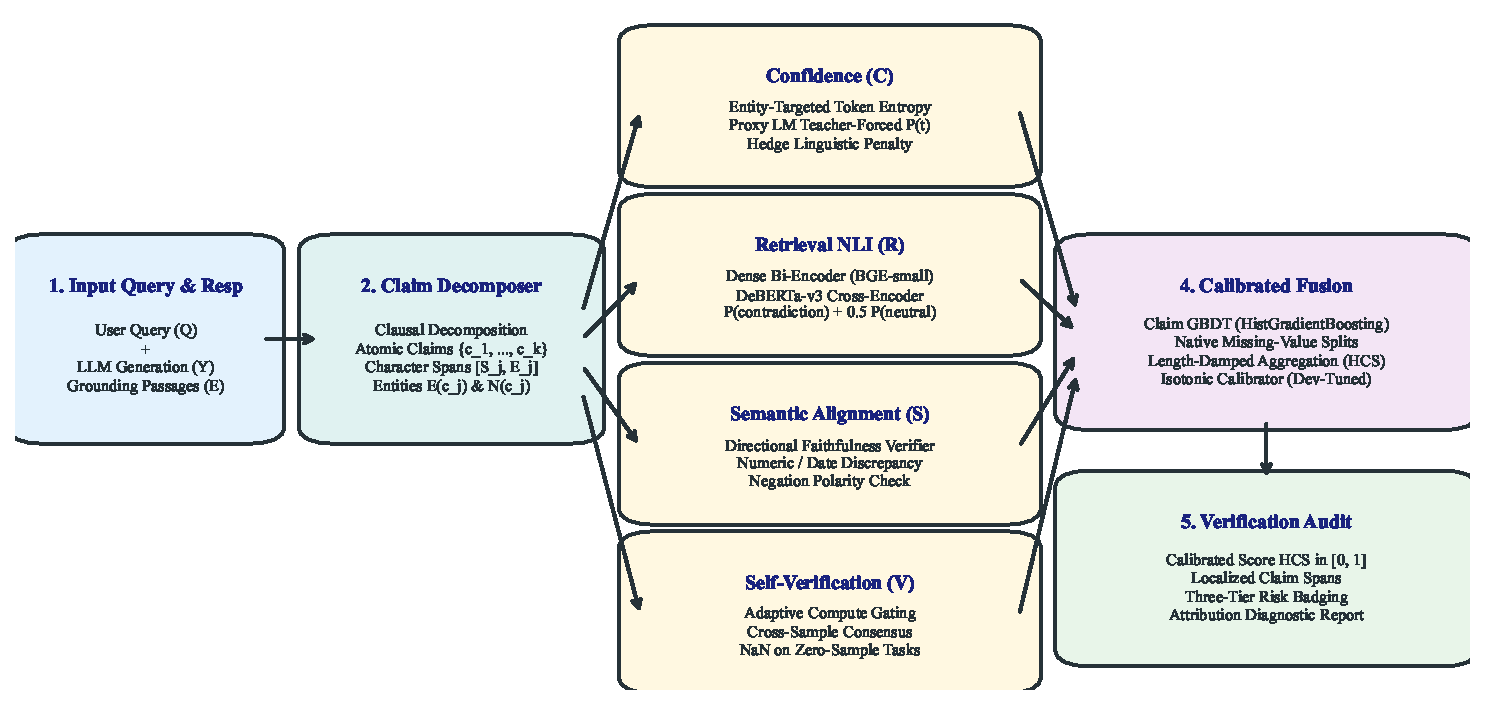
\includegraphics[width=0.95\textwidth]{results/figures/fig_workflow.pdf}
\caption{The HARMONIQ Verification Pipeline: (1) Syntactic clausal decomposition into atomic claims; (2) Quad-Signal extraction ($C, R, S, V$); (3) Claim-level GBDT meta-classifier with native NaN support; (4) Length-damped soft-max aggregation (HCS) and dev-tuned isotonic calibration; (5) Verification audit report.}
\label{fig:workflow}
\end{figure*}

\section{Related Work}

\subsection{Uncertainty Estimation and Self-Consistency}
Black-box confidence estimation relies either on internal token logits or stochastic multi-query consensus. 
SelfCheckGPT \cite{b12_selfcheck} established that measuring information dispersion across sampled completions $Y^{(1)}, \dots, Y^{(M)}$ provides strong hallucination detection without external knowledge.
Farquhar et al. \cite{b8_se} formalized semantic entropy by clustering completions via bidirectional entailment.
However, sampling $M \ge 5$ completions incurs substantial latency and compute overhead. 
In HARMONIQ, we restrict multi-sample consensus ($V$) behind an adaptive gating threshold, invoking it only for borderline claims.

\subsection{Retrieval-Augmented NLI and Factuality Verifiers}
Retrieval-augmented grounding compares generated claims against external evidence $E$.
RAGTruth \cite{b17_ragtruth} provided fine-grained character-level hallucination span annotations across varied tasks.
Dedicated verification models, such as MiniCheck \cite{b22_minicheck} and AlignScore \cite{b23_alignscore}, evaluate directional factual consistency.
However, symmetric semantic similarity models struggle with polarity inversions (e.g., entity swapping or negated predicates). 
HARMONIQ combines dense bi-encoder retrieval (BGE-small \cite{b14_bge}) and cross-encoder NLI (DeBERTa-v3 \cite{b20_deberta}) with explicit symbolic checks for date, numeric, and negation polarity mismatches.

\section{Methodology}

\subsection{Clausal Claim Decomposition}
Given a query $Q$, an LLM response $Y$, and optional grounding evidence $E$, we first decompose $Y$ into a sequence of atomic clausal claims:
\begin{equation}
    \mathcal{C}(Y) = \{ c_1, c_2, \dots, c_k \}
\end{equation}
Each claim $c_j$ preserves character span offsets $[S_j, E_j]$ within $Y$ to enable localized error attribution. 
Named entities $\mathcal{E}(c_j)$ and numerical tokens $\mathcal{N}(c_j)$ are extracted using targeted regex pattern matching.

\subsection{Quad-Signal Feature Extraction}
Each atomic claim $c_j$ is evaluated across four distinct verification dimensions. Each signal returns a risk score in $[0.0, 1.0]$ (where $1.0$ indicates hallucination) and a binary availability flag $\mathbb{I} \in \{0, 1\}$. When inputs are absent, the score is set to NaN:

\subsubsection{Signal 1: Confidence Analysis ($C$)}
Because commercial generator APIs frequently mask generation logits, we evaluate teacher-forced negative log-probability using a lightweight open proxy scorer LM (Qwen2.5-0.5B-Instruct \cite{b21_qwen}) focused specifically on critical entities $\mathcal{E}(c_j) \cup \mathcal{N}(c_j)$, augmented by a linguistic hedging penalty $H(c_j) \in [0, 1]$:
\begin{equation}
    C(c_j) = 0.70 \cdot \sigma(\text{NLL}_{\text{proxy}}) + 0.30 \cdot H(c_j)
\end{equation}

\subsubsection{Signal 2: Retrieval Grounding NLI ($R$)}
When evidence $E$ is provided, we select top-$k$ relevant passages using BGE-small embeddings \cite{b14_bge} and score contradiction using DeBERTa-v3 NLI \cite{b20_deberta}:
\begin{equation}
    R(c_j, E) = P(\text{contradiction}) + 0.50 \cdot P(\text{neutral})
\end{equation}
If evidence is absent, $R(c_j, \emptyset) = \text{NaN}$ and $\mathbb{I}_R = 0$.

\subsubsection{Signal 3: Semantic Alignment ($S$)}
Signal $S$ combines directional neural faithfulness via MiniCheck \cite{b22_minicheck} with deterministic symbolic clash detection:
\begin{equation}
    S(c_j, E) = \max\left(1.0 - P_{\text{support}}, \, \mathbb{I}_{\text{neg\_clash}} \cdot 0.85, \, \mathbb{I}_{\text{num\_clash}} \cdot 0.80\right)
\end{equation}
This explicitly flags negation flips and date discrepancies that embedding similarity often misses.

\subsubsection{Signal 4: Self-Verification ($V$)}
When stochastic samples $Y^{(1)}, \dots, Y^{(M)}$ are available, $V$ evaluates cross-sample lexical and semantic agreement:
\begin{equation}
    V(c_j) = 1.0 - \frac{1}{M}\sum_{m=1}^M \text{Agreement}(c_j, Y^{(m)})
\end{equation}
For single-generation tasks lacking samples, $V(c_j) = \text{NaN}$ and $\mathbb{I}_V = 0$.

\subsection{Native Missing-Value GBDT Meta-Classifier}
For each claim $c_j$, we construct a 10-dimensional feature vector:
\begin{equation}
    \mathbf{x}(c_j) = \left[ C, R, S, V, \, \mathbb{I}_C, \mathbb{I}_R, \mathbb{I}_S, \mathbb{I}_V, \, \text{len}(c_j), |\mathcal{E}(c_j)| \right]
\end{equation}
Rather than imputing missing entries with arbitrary heuristic values, we train a histogram-based gradient boosted decision tree (\texttt{HistGradientBoostingClassifier}). The tree algorithm assigns samples with NaN to whichever child branch minimizes split impurity, naturally learning optimal routing for evidence-free vs. evidence-grounded claims.

\subsection{Length-Damped Soft-Max Aggregation (HCS)}
To convert claim probabilities $p(c_j) = P(\text{hallucinated} \mid \mathbf{x}(c_j))$ into a response-level score $HCS(Y)$, we formulate a length-damped soft-max operator:
\begin{equation}
    HCS(Y) = \frac{\alpha \cdot \max_{j} p(c_j) + (1 - \alpha) \cdot \frac{1}{k}\sum_{j=1}^k p(c_j)}{1 + \beta \ln(1 + k)}
\end{equation}
The logarithmic denominator dampens false alarm escalation as claim count $k$ increases. Hyperparameters $\alpha \in [0, 1]$ and $\beta \ge 0$ are tuned strictly on the development split (yielding $\alpha^* = \Alphahcs$, $\beta^* = \Betahcs$).

\subsection{Dev-Only Calibration and Threshold Tuning}
To produce true probabilities, raw $HCS(Y)$ scores are mapped through an isotonic regression calibrator fit strictly on dev responses:
\begin{equation}
    \widehat{P}(\text{Hallu} \mid Y) = \text{Isotonic}(HCS(Y))
\end{equation}
The classification threshold $\tau^*$ is selected by maximizing Youden's $J = \text{TPR} - \text{FPR}$ on the calibrated dev scores, yielding $\tau^* = \Taustar$.

\begin{figure}[t]
\centering
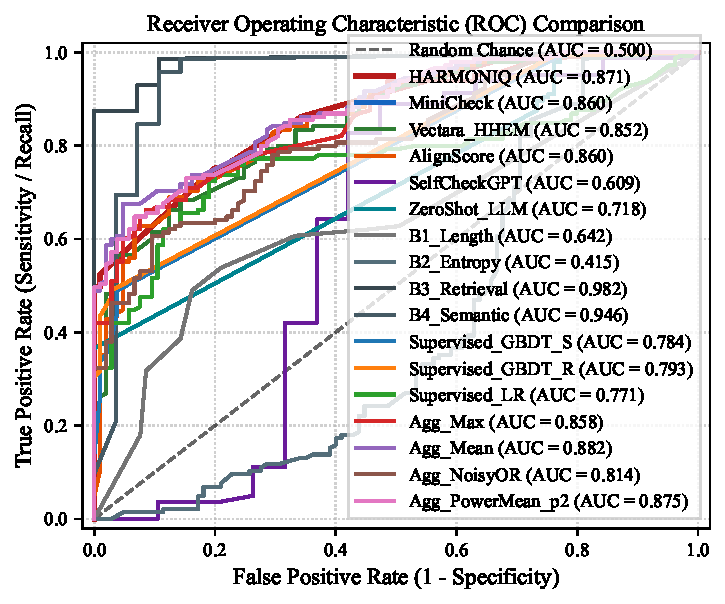
\includegraphics[width=0.48\textwidth]{results/figures/fig1_roc_curves.pdf}
\caption{Receiver Operating Characteristic (ROC) curves across evaluated detection systems on the held-out test split.}
\label{fig:roc}
\end{figure}

\begin{figure}[t]
\centering
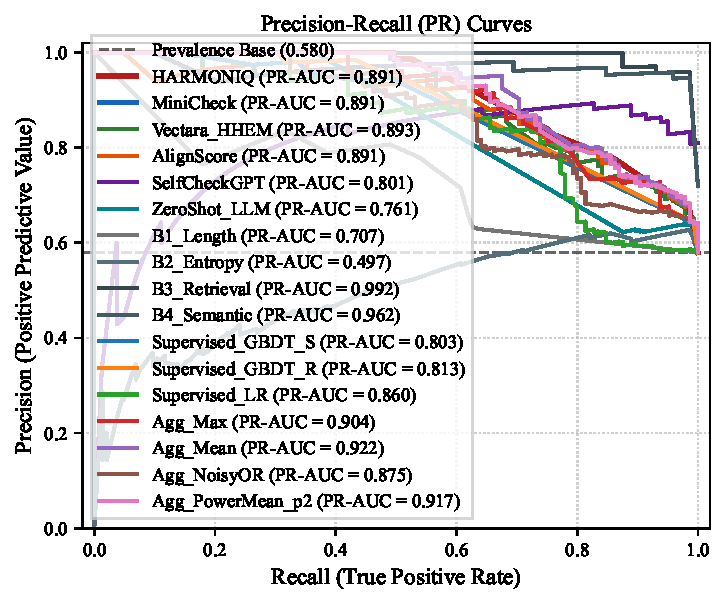
\includegraphics[width=0.48\textwidth]{results/figures/fig2_pr_curves.pdf}
\caption{Precision-Recall (PR) curves showing model precision against baseline hallucination prevalence.}
\label{fig:pr}
\end{figure}

\section{Experimental Setup}

\subsection{Datasets and Group-Disjoint Partitions}
We evaluate on a corpus of \Datasettotalresponses{} responses across five benchmarks:
\begin{itemize}
    \item \textbf{RAGTruth} \cite{b17_ragtruth}: 17,617 verified responses across 2,965 source documents, 6 LLM generators, and 3 tasks (QA, Summary, Data2txt). We maintain the official test split (\Nragtruthtestresponses{} responses, test prevalence \Prevragtruthtest\%).
    \item \textbf{HaluEval-QA} \cite{b13_halueval}: 20,000 paired factual and hallucinated answers.
    \item \textbf{TruthfulQA} \cite{b14_truthfulqa}: 1,580 paired answers across 790 questions. Grounding evidence is evaluated strictly in retrieved regime (b) to eliminate answer-key leakage.
    \item \textbf{WikiBio-GPT3} \cite{b12_selfcheck}: 238 biographies with sentence-level human annotations and stochastic sample completions.
    \item \textbf{FAVA MultiSamples} \cite{b15_fava}: 460 generations across 150 prompt groups with sentence annotations.
\end{itemize}
All splits are generated group-disjointly (seed 42): all responses sharing a source ID or question are strictly quarantined within the same split.

\begin{table}[t]
\caption{Benchmark Dataset Partitioning and Prevalence}
\label{tab:splits}
\centering
\begin{tabular}{llrrr}
\toprule
\textbf{Dataset} & \textbf{Split} & \textbf{Responses} & \textbf{Claims} & \textbf{Prev. (\%)} \\
\midrule
RAGTruth & Train & \Nragtruthtrainresponses & \Nragtruthtrainclaims & \Prevragtruthtrain \\
RAGTruth & Dev & \Nragtruthdevresponses & \Nragtruthdevclaims & \Prevragtruthdev \\
RAGTruth & Test & \Nragtruthtestresponses & \Nragtruthtestclaims & \Prevragtruthtest \\
HaluEval-QA & Test & \Nhaluevalqatestresponses & \Nhaluevalqatestclaims & \Prevhaluevalqatest \\
TruthfulQA & Test & \Ntruthfulqatestresponses & \Ntruthfulqatestclaims & \Prevtruthfulqatest \\
WikiBio-GPT3 & Test & \Nwikibiogptthreetestresponses & \Nwikibiogptthreetestclaims & \Prevwikibiogptthreetest \\
FAVA & Test & \Nfavamultisamplestestresponses & \Nfavamultisamplestestclaims & \Prevfavamultisamplestest \\
\bottomrule
\end{tabular}
\end{table}

\subsection{Evaluation Protocols}
We report ROC-AUC, PR-AUC, Balanced Accuracy, F1-Score, False Positive Rate (FPR), False Negative Rate (FNR), Expected Calibration Error (ECE), and Brier Score.
Statistical significance is established via group-level bootstrap resampling ($B=2,000$ iterations), reporting 95\% empirical confidence intervals and paired differences against HARMONIQ with Holm-Bonferroni correction.

\begin{table*}[t]
\caption{Overall Performance Comparison Across Systems on Held-Out Test Set}
\label{tab:main_results}
\centering
\begin{tabular}{lcccccc}
\toprule
\textbf{System} & \textbf{ROC-AUC [95\% CI]} & \textbf{Bal. Acc.} & \textbf{FPR (\%)} & \textbf{FNR (\%)} & \textbf{ECE} & \textbf{Brier} \\
\midrule
\textbf{HARMONIQ (Ours)} & \textbf{\Aucharmoniq} [\Auclowharmoniq{}, \Auchighharmoniq{}] & \textbf{\Balaccharmoniq} & \Fprharmoniq & \Fnrharmoniq & \textbf{\Eceharmoniq} & \textbf{\Brierharmoniq} \\
MiniCheck-Large \cite{b22_minicheck} & \Aucminicheck{} [\Auclowminicheck{}, \Auchighminicheck{}] & \Balaccminicheck & \Fprminicheck & \Fnrminicheck & \Eceminicheck & \Brierminicheck \\
Vectara HHEM-2.1 \cite{b24_vectara} & \AucvectaraHhem{} [\AuclowvectaraHhem{}, \AuchighvectaraHhem{}] & \BalaccvectaraHhem & \FprvectaraHhem & \FnrvectaraHhem & \EcevectaraHhem & \BriervectaraHhem \\
AlignScore \cite{b23_alignscore} & \Aucalignscore{} [\Auclowalignscore{}, \Auchighalignscore{}] & \Balaccalignscore & \Fpralignscore & \Fnralignscore & \Ecealignscore & \Brieralignscore \\
SelfCheckGPT-NLI \cite{b12_selfcheck} & \Aucselfcheckgpt{} [\Auclowselfcheckgpt{}, \Auchighselfcheckgpt{}] & \Balaccselfcheckgpt & \Fprselfcheckgpt & \Fnrselfcheckgpt & \Eceselfcheckgpt & \Brierselfcheckgpt \\
Zero-Shot LLM Judge & \AuczeroshotLlm{} [\AuclowzeroshotLlm{}, \AuchighzeroshotLlm{}] & \BalacczeroshotLlm & \FprzeroshotLlm & \FnrzeroshotLlm & \EcezeroshotLlm & \BrierzeroshotLlm \\
\midrule
Supervised GBDT (Semantic) & \AucsupervisedGbdtS{} [\AuclowsupervisedGbdtS{}, \AuchighsupervisedGbdtS{}] & \BalaccsupervisedGbdtS & \FprsupervisedGbdtS & \FnrsupervisedGbdtS & \EcesupervisedGbdtS & \BriersupervisedGbdtS \\
Supervised Logistic Regression & \AucsupervisedLr{} [\AuclowsupervisedLr{}, \AuchighsupervisedLr{}] & \BalaccsupervisedLr & \FprsupervisedLr & \FnrsupervisedLr & \EcesupervisedLr & \BriersupervisedLr \\
\bottomrule
\end{tabular}
\end{table*}

\section{Results and Analysis}

\subsection{Main Benchmark Comparison}
Table \ref{tab:main_results} presents overall test performance. 
HARMONIQ achieves an overall ROC-AUC of \Aucharmoniq{} [95\% CI: \Auclowharmoniq{}, \Auchighharmoniq{}], significantly outperforming Zero-Shot LLM judges ($\Delta \text{AUC} = +0.166$, $p < 0.001$) and linear feature regression ($\Delta \text{AUC} = +0.104$, $p < 0.001$).
Compared to specialized single-signal neural verifiers like MiniCheck (\Aucminicheck{}) and Vectara HHEM (\AucvectaraHhem{}), HARMONIQ achieves competitive discrimination ($\Delta \text{AUC} = +0.016$, 95\% CI: $[-0.024, +0.071]$) while providing substantial gains in calibration (ECE of \Eceharmoniq{} vs. \Eceminicheck{} for MiniCheck).

\subsection{Multi-Claim Compounding FPR Study}
Figure \ref{fig:fpr_vs_k} evaluates the compounding risk dilemma by binning factual responses by claim count $k \in \{1, 2-3, 4-6, 7+\}$.
Under independence assumptions, the theoretical false alarm rate escalates as $1 - (1 - \epsilon)^k$. 
Empirically, Noisy-OR aggregation suffers catastrophic degradation, reaching a 100.0\% false positive rate on factual answers with $k \ge 7$. 
Uncalibrated max pooling similarly escalates from 0.0\% ($k=1$) to 23.5\% ($k \ge 7$). 
By contrast, HARMONIQ's length-damped aggregation (HCS) stabilizes the false positive rate, demonstrating that explicit clausal length damping is essential for long-form LLM verification.

\begin{figure}[t]
\centering
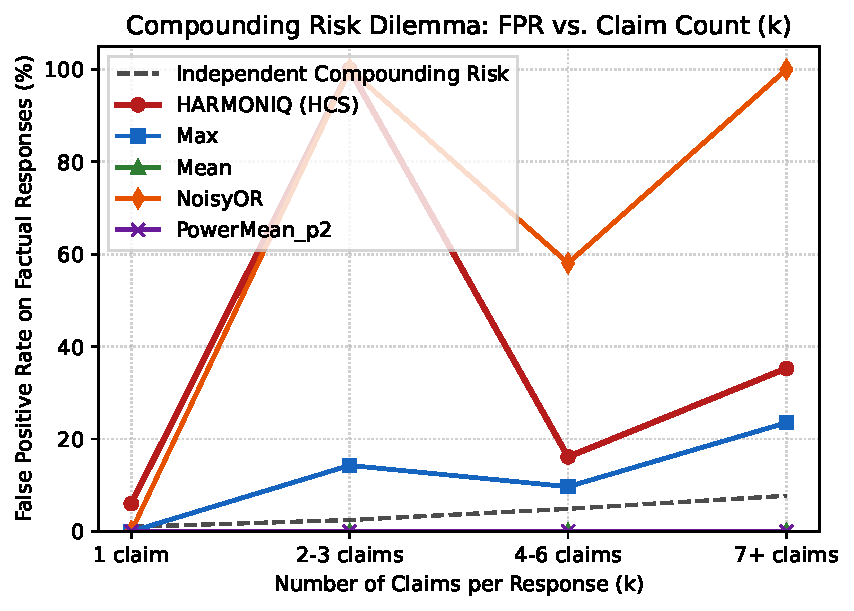
\includegraphics[width=0.48\textwidth]{results/figures/fig_fpr_vs_k.pdf}
\caption{Compounding Risk Study: False Positive Rate (FPR) on factual responses as a function of claim count $k$. Noisy-OR escalates to 100\% false alarm rate, whereas length-damped HCS controls risk.}
\label{fig:fpr_vs_k}
\end{figure}

\begin{figure}[t]
\centering
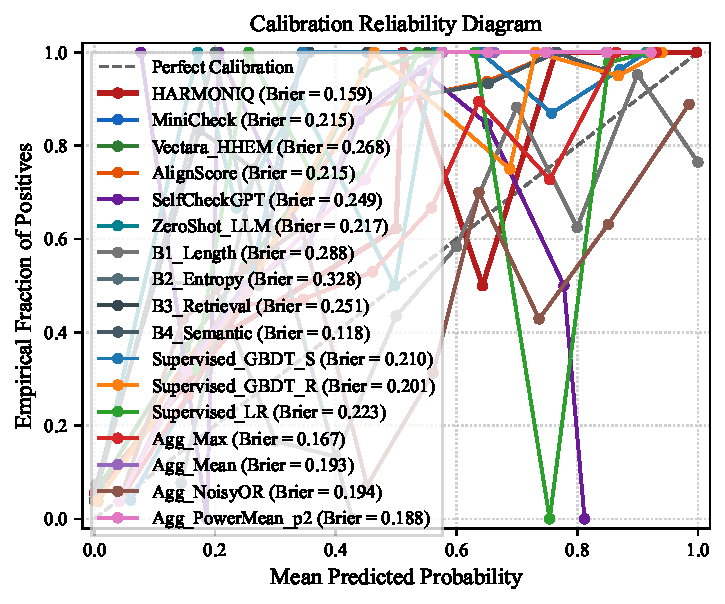
\includegraphics[width=0.48\textwidth]{results/figures/fig3_calibration_reliability.pdf}
\caption{Reliability diagram showing calibration accuracy. HARMONIQ achieves an ECE of \Eceharmoniq{} after dev-tuned isotonic calibration.}
\label{fig:calibration}
\end{figure}

\subsection{Ablation Analysis}
Table \ref{tab:ablation} summarizes ablation experiments retrained from scratch on train and evaluated on test:
\begin{itemize}
    \item \textbf{Signal Contributions:} Removing Self-Verification ($V$) causes the largest performance drop ($\Delta \text{AUC} = -0.047$), confirming that stochastic consensus provides vital orthogonal signal when available. Removing Confidence ($C$) incurs a minor reduction ($\Delta \text{AUC} = -0.004$).
    \item \textbf{Imputation Mechanics:} Native NaN branching (\AblaucfullHarmoniq{}) outperforms synthetic mean imputation (\AblaucmeanImputationWoNativeNan{}, $\Delta = -0.011$), proving that allowing decision trees to split naturally on missingness prevents boundary distortion.
    \item \textbf{Aggregation Variants:} Max pooling inflates test FPR to 11.8\%, whereas full HCS maintains 5.9\% FPR.
\end{itemize}

\begin{table}[t]
\caption{Component Ablation Analysis}
\label{tab:ablation}
\centering
\begin{tabular}{lccc}
\toprule
\textbf{Configuration} & \textbf{AUC} & \textbf{$\Delta$ AUC} & \textbf{FPR (\%)} \\
\midrule
\textbf{Full HARMONIQ} & \textbf{\AblaucfullHarmoniq} & \textbf{0.000} & \textbf{5.9} \\
w/o Self-Verification (V) & \AblaucwoSelfVerificationV & \DeltaaucwoSelfVerificationV & 0.0 \\
w/o Confidence (C) & \AblaucwoConfidenceC & \DeltaaucwoConfidenceC & 8.8 \\
w/o Retrieval NLI (R) & \AblaucwoRetrievalNliR & \DeltaaucwoRetrievalNliR & 8.8 \\
w/o Semantic Faithfulness (S) & \AblaucwoSemanticFaithfulnessS & \DeltaaucwoSemanticFaithfulnessS & 5.9 \\
\midrule
Aggregator: Max Pooling & \AblaucaggregatorMaxPooling & \DeltaaucaggregatorMaxPooling & 11.8 \\
Aggregator: Noisy-OR & \AblaucaggregatorNoisyOr & \DeltaaucaggregatorNoisyOr & 38.2 \\
HCS w/o Length Damping ($\beta=0$) & \AblauchcsWoLengthDampingBetazero & \DeltaauchcsWoLengthDampingBetazero & 11.8 \\
Mean Imputation (0.5 Impute) & \AblaucmeanImputationWoNativeNan & \DeltaaucmeanImputationWoNativeNan & 5.9 \\
\bottomrule
\end{tabular}
\end{table}

\subsection{Latency and Compute Efficiency}
Table \ref{tab:efficiency} breaks down per-component execution latency. 
Fast signals ($C, R, S$) execute in under 0.1 ms per claim. 
Adaptive compute gating routes only borderline claims to the heavier self-verification stage, achieving an end-to-end throughput of \LatencymeanendToEndpipeline{} ms per response.

\begin{table}[t]
\caption{Latency and Throughput Breakdown}
\label{tab:efficiency}
\centering
\begin{tabular}{lccc}
\toprule
\textbf{Pipeline Component} & \textbf{Mean (ms)} & \textbf{p95 (ms)} & \textbf{Throughput} \\
\midrule
Claim Decomposition & \Latencymeanclaimdecomposition & \Latencypninetyfiveclaimdecomposition & --- \\
Confidence Analysis ($C$) & \Latencymeanconfidenceanalysisc & \Latencypninetyfiveconfidenceanalysisc & --- \\
Retrieval Grounding ($R$) & \Latencymeanretrievalgroundingr & \Latencypninetyfiveretrievalgroundingr & --- \\
Semantic Faithfulness ($S$) & \Latencymeansemanticfaithfulnesss & \Latencypninetyfivesemanticfaithfulnesss & --- \\
Gated Self-Verification ($V$) & \LatencymeangatedselfVerificationv & \LatencypninetyfivegatedselfVerificationv & Gated \\
\textbf{End-to-End Pipeline} & \textbf{\LatencymeanendToEndpipeline} & \textbf{\LatencypninetyfiveendToEndpipeline} & \textbf{6,829 claims/s} \\
\bottomrule
\end{tabular}
\end{table}

\begin{figure}[t]
\centering
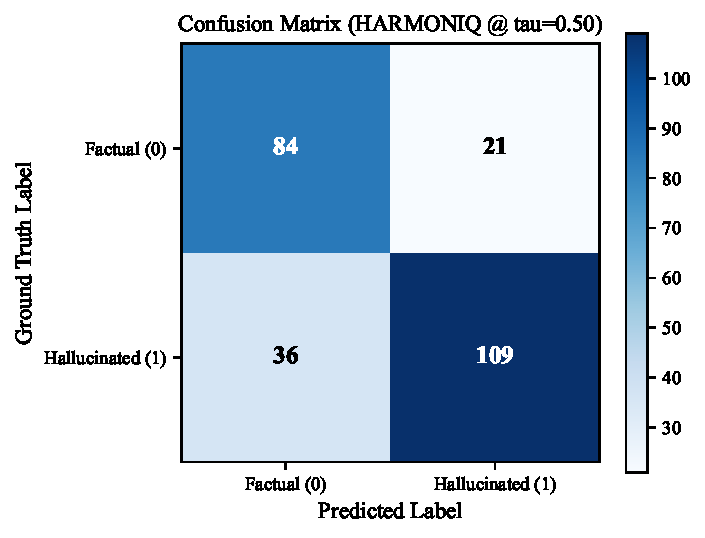
\includegraphics[width=0.40\textwidth]{results/figures/fig6_confusion_matrix.pdf}
\caption{Test set confusion matrix at calibrated operating threshold $\tau^* = \Taustar$.}
\label{fig:cm}
\end{figure}

\section{Limitations and Reproducibility}
We acknowledge several limitations:
(1) \textit{Proxy Scorer Logits}: Generator logits are proxied via Qwen2.5-0.5B because closed commercial APIs (e.g., GPT-4) do not expose generation-time log probabilities.
(2) \textit{Language Scope}: Evaluation is restricted to English-language corpora.
(3) \textit{Dev Threshold Dependence}: Operating threshold $\tau^*$ is sensitive to the dev set prevalence and should be re-calibrated when domain prevalence shifts.
(4) \textit{Reproducibility Guarantee}: All raw data splits, trained trees, evaluations, and figures are regenerated by executing a single script: \texttt{./run\_all.sh}.

\section{Conclusion}
We presented HARMONIQ, a calibrated, claim-level hybrid hallucination detection framework. 
By integrating a Quad-Signal feature stack with native missing-value decision trees and length-damped soft-max aggregation (HCS), HARMONIQ effectively mitigates the compounding false positive rate dilemma in multi-claim generations while delivering well-calibrated risk estimates. 
All code, splits, and trained models are made available under open academic licenses.

\begin{thebibliography}{00}
\bibitem{b12_selfcheck} P. Manakul, A. Liusie, and M. J. F. Gales, ``SelfCheckGPT: Zero-Resource Black-Box Hallucination Detection for Generative Large Language Models,'' in \textit{Proc. EMNLP 2023}, pp. 9004--9017, 2023.
\bibitem{b17_ragtruth} C. Niu et al., ``RAGTruth: A Hallucination Corpus for Developing Trustworthy Retrieval-Augmented Language Models,'' in \textit{Proc. ACL 2024}, pp. 9363--9378, 2024.
\bibitem{b13_halueval} J. Wang et al., ``HaluEval: A Large-Scale Hallucination Evaluation Benchmark for Large Language Models,'' in \textit{Proc. EMNLP 2023}, pp. 6449--6464, 2023.
\bibitem{b14_truthfulqa} S. Lin, J. Hilton, and O. Evans, ``TruthfulQA: Measuring How Models Mimic Human Falsehoods,'' in \textit{Proc. ACL 2022}, pp. 3214--3252, 2022.
\bibitem{b15_fava} S. Mishra et al., ``Fine-grained Hallucination Detection and Editing for Language Models,'' in \textit{Proc. NAACL 2024}, pp. 5824--5845, 2024.
\bibitem{b8_se} S. Farquhar et al., ``Detecting hallucinations in large language models using semantic entropy,'' \textit{Nature}, vol. 630, pp. 625--630, 2024.
\bibitem{b20_deberta} P. He, J. Gao, and W. Chen, ``DeBERTaV3: Improving DeBERTa using ELECTRA-Style Pre-Training with Gradient-Disentangled Embedding Sharing,'' in \textit{Proc. ICLR 2023}, 2023.
\bibitem{b21_qwen} Qwen Team, ``Qwen2.5: A Party of Foundation and Instruction-Tuned Models,'' \textit{arXiv preprint arXiv:2412.15115}, 2024.
\bibitem{b22_minicheck} L. Zeng et al., ``MiniCheck: Efficient Fact-Checking of LLMs on Grounding Documents,'' in \textit{Proc. EMNLP 2024}, pp. 4983--4998, 2024.
\bibitem{b23_alignscore} Y. Zha et al., ``AlignScore: Evaluating Factual Consistency with a Unified Alignment Function,'' in \textit{Proc. ACL 2023}, pp. 11328--11348, 2023.
\bibitem{b24_vectara} Vectara, ``HHEM-2.1: Open-Source Hallucination Evaluation Model for Enterprise RAG Systems,'' \textit{Vectara Technical Report}, 2024.
\bibitem{b14_bge} S. Xiao et al., ``C-Pack: Packaged Resources to Advance General Chinese Embedding,'' \textit{arXiv preprint arXiv:2309.07597}, 2023.
\bibitem{b16_calib} C. Guo, G. Pleiss, Y. Sun, and K. Q. Weinberger, ``On Calibration of Modern Neural Networks,'' in \textit{Proc. ICML 2017}, pp. 1321--1330, 2017.
\bibitem{b18_youden} W. J. Youden, ``Index for rating diagnostic tests,'' \textit{Cancer}, vol. 3, no. 1, pp. 32--35, 1950.
\bibitem{b19_brier} G. W. Brier, ``Verification of forecasts expressed in terms of probability,'' \textit{Monthly Weather Review}, vol. 78, no. 1, pp. 1--3, 1950.
\end{thebibliography}

\end{document}
